
\documentclass[12pt,a4paper]{article}

\usepackage{fontspec}

\usepackage[BoldFont]{xeCJK}

%\setCJKmainfont{BiauKaiTC}                % 中文字型使用標楷體
\setCJKmainfont{DFKai-SB}
\setmainfont{Times New Roman}          % 如果英文字型是 Times New Roman 則取消這行註解

\XeTeXlinebreaklocale "zh"             % 這兩行一定要加,中文才能自動換行

\XeTeXlinebreakskip = 0pt plus 1pt     % 這兩行一定要加,中文才能自動換行

\usepackage{geometry}

\geometry{
a4paper,
left=27mm,       %左邊界
right=27mm,      %右邊界
top=20mm,        %上邊界
bottom=12mm,     %下邊界
 }

\usepackage{amssymb}

\usepackage{mathtools}

\usepackage{microtype}

\usepackage{enumitem}

\usepackage{dirtytalk}

\usepackage{subcaption}

\usepackage{fancyhdr}

\usepackage{graphicx}

\usepackage{indentfirst}

\usepackage{hyperref}

\usepackage{zhnumber}

\zhnumsetup{style=Traditional}

\usepackage[backend=biber,style=ieee]{biblatex}

\addbibresource{references.bib}

\AddEnumerateCounter{\zhdig}{\zhdig}{}

\DeclareCaptionLabelSeparator{custom}{、 }

\usepackage[justification=centering,figurename={},tablename={},labelsep=custom]{caption}

\renewcommand{\thetable}{表\zhdig{table}}

\renewcommand{\thefigure}{圖\zhdig{figure}}

\renewcommand{\tableautorefname}{}

\pagestyle{fancy}

\fancyhead{} % 清除所有頁首設定

\fancyfoot{}

\renewcommand{\headrulewidth}{0pt}

\renewcommand{\footrulewidth}{0pt}

\setlength{\headwidth}{\textwidth}

\lfoot{表 C802}

\rfoot{共~~\pageref{LastPage}~~頁~~第{~~\thepage~~}頁}

\begin{document}

\setlength{\parindent}{2em}

\noindent{\bf \large  二、 研究計畫內容:}

\begin{enumerate}[label={(\zhdig*)}, leftmargin=2\parindent, listparindent=\parindent]

\item 摘要

本研究計畫以「預測先行、服務水準協議 (Service-Level Agreement, SLA) 驅動與智能調度」
三大核心手段,針對高併發應用程式介面 (Application Program Interface, API) 服務所面臨的資
源調度與負載激增問題,提出一套整合深度學習、
強化學習與容器編排的智能化系統,透過卷積神經網路 (Convolutional Neural Network, CNN)
與長短期記憶模型 (Long Short-Term Memory, LSTM) 進行集群與 Pod 層級的負載預測,以達
到主動式擴縮集群的目的,避免因其而造成的服務延遲或中斷。

系統額外加入了多重動態門檻監控模組,
透過監控 CPU、記憶體使用率、API 響應時間
與請求成功率等指標,協助動態調整 SLA 閾值,
並為了讓 Pod 分配至最佳節點以提升資源利用率
與降低延遲,整合元啟發式演算法優化
Kubernetes 的排程器 (Scheduler)。

此外,系統中的自適應
集群擴縮模組與特別加入的冷卻機制,可根據負載
預測結果和服務級別目標 (Service-level objective, SLO),動態增減叢集節點與容器
數量與避免頻繁震盪。

此架構不僅可應用於電商促銷、金融交易及 IoT
感測等多樣場景,也能確保 SLA 指標穩定達成並
有效控制雲端成本。

\item 研究動機與研究問題

\begin{enumerate}[label={(\arabic*)}, leftmargin=\parindent, listparindent=\parindent]

\item\textbf{研究問題}

隨著微服務 (Microservices)\cite{1}和雲端原生技術
(Cloud-Native)\cite{2}的普及,現代應用系統高度依
賴高併發應用程式介面 (Application Program Interface, API)
服務,應用於金融交易、電商促銷、影音串流、物聯網等場景,並對 低延遲、
高可用性與動態擴展提出了嚴格要求。例如:

\begin{itemize}[leftmargin=\parindent, listparindent=\parindent]

\item 金融交易 API 需要毫秒級延遲來確保最佳買賣時機,對資源調度
與計算負載有極高要求。交易峰值可能在短短幾秒內增加數十倍,若 API
擴展反應過慢,可能導致交易失敗或市場損失。\cite{3}

\item 大型電商平台促銷活動期間 (如雙 11 促銷活動),大量用戶同時
請求API 進行商品查詢、購物車更新、訂單提交,瞬間請求量可達數百萬每
秒查詢數 (Queries Per Second, QPS)。傳統的 API 擴展方式無法即
時應對流量暴增,可能導致購物車服務崩潰、支付 API 超時,影響用戶體驗
與企業營收。\cite{4}

\item 社群媒體與影音串流 (如 TikTok、YouTube、Instagram)
用戶大量發送請求以獲取動態、影片內容,並伴隨 AI 推薦計算
(如 TikTok For You Feed)。服務需要即時擴展,確保推播
內容的低延遲傳遞,同時兼顧後端機器學習推理任務的負載平衡。\cite{5}

\item 物聯網 (Internet of Things, IoT) 平台
(如智慧城市、工業 4.0) 則是有大量 IoT 設備持續發
送感測數據至雲端 API 進行分析、存儲,且流量具有明
顯的時段性波動 (如白天比晚上流量高)。若 API 無法
適應 IoT 端的流量模式,可能導致數據擷取延遲或設備
無法連接雲端,影響關鍵應用 (如智慧交通信號調度)。\cite{6}

\end{itemize}

然而,目前有許多企業採用 Kubernetes (K8s) 來管理雲端資源,
並透過 Pod 水平/垂直自動擴縮器
(Horizontal/Vertical Pod Autoscaler, H/VPA)
和集群自動擴縮器 (Cluster Autoscaler, CA)
來應對流量變化。然而,這些現有擴展機制在高併發 API
服務場景下仍存在以下關鍵問題\cite{7}:
\begin{itemize}[leftmargin=\parindent, listparindent=\parindent]
    \item\textbf{資源調度延遲:}

H/VPA 依賴中央處理器 (CPU) 或記憶體的用量閾值來監測並觸發 Pod 擴縮,
然而這種方式屬於被動式反應,H/VPA 需要等到 CPU 或記憶體負載超過閾值
後才開始擴展,這意味著系統已經開始過載才會進行調整,並且 H/VPA 整體
擴展過程也會具有一定延遲,從而導致 API 服務短期內請求失敗率上升。

    \item \textbf{
負載預測不準確
}

H/VPA 無法提前預測 API 流量模式,而是單純依賴當下的 CPU 或記憶體使用率,
這在應對突發性高併發流量時顯得效率低下,例如電商促銷開始前的
API 請求量通常會呈指數級增長,但 H/VPA 在負載真正升高前不
會觸發擴展,導致初期請求可能被拒絕。

\item \textbf{無法學習歷史數據:}

H/VPA 不會根據歷史 流量模式來調整策略,無法針對每天固定時段的高峰流量 (如午餐時段、晚間流量高峰)
做出提前擴展的決策。

    \end{itemize}
    \item \textbf{研究動機與目標}

容器調度 (Container Scheduling) 是雲端計算和邊緣計算領域的重要研究
課題,其目標是在動態環境中有效管理資源,確保負載均衡、降低能源消耗
並提升應用效能。現有的研究方法\cite{11}可分為\textbf{數學建模 (Mathematical
Modeling) 、啟發式演算法 (Heuristic Algorithms) 、
元啟發式演算法 (MetaHeuristic Algorithms) 、
機器學習 (Machine Learning) }等不同類別,本節
將基於近期的研究成果進行綜合探討與比較。

\begin{enumerate}[label={(\zhdig*)}, leftmargin=\parindent, listparindent=\parindent]

\item \textbf{啟發式演算法:區域性感知與多目標調度}

啟發式演算法通常透過經驗法則和啟發資訊進行資源分配,較適用於即
時調度需求,但易受局部最優解影響。
\begin{itemize}[leftmargin=\parindent, listparindent=\parindent]
    \item \textbf{
        \cite{12} 區域性感知 (Locality-Aware) 調度}

    Diego 等人提出了一種區域性感知的調度機制,透過
    統計方法將負載均衡 (Load Balancing) 與應用效能 (Application Performance)
    統一為一個優化問題,以降低 I/O 和網路流量瓶頸。該方法適用於資料密
    集型應用,並在 CloudFoundry 平台上驗證了其效能優勢。
    \item \textbf{\cite{13} Multiopt:多目標最佳化調度}

    Multiopt 是一種基於多目標最佳化 (Multi-Objective Optimization) 的調
    度方法,綜合考量 CPU 使用率、記憶體使用率、網路傳輸時間、容器與節
    點的關聯性、容器聚類等五個因素,透過計分函數 (Scoring Function) 選
    擇最佳節點來部署容器,進一步提高系統的每
    秒交易數 (Transactions Per Second, TPS) 並降低平均響應時間。

\end{itemize}
\item \textbf{
    元啟發式演算法:螞蟻、粒子群與混合演算法
}

元啟發式演算法 (Meta-Heuristic Algorithms) 利用啟發資訊進行全域搜
尋,適用於複雜調度問題,但計算開銷較高。
\begin{itemize}[leftmargin=\parindent, listparindent=\parindent]
    \item \textbf{\cite{14} MOO-ACA,GA-MOCA:基於螞蟻演算法 (ACO) 的容器調度}

    MOO-ACA 透過螞蟻演算法 (Ant Colony Algorithm, ACO) 來考量網路
    傳輸開銷、負載均衡與服務可靠性,運用費洛蒙更新機制提升全域最適性,
    使得容器調度更符合雲端環境的變動需求。

    \item \textbf{
        \cite{15} EECS 與 APSO:基於粒子群最佳化的能效調度
    }

    EECS 採用加速粒子群最佳化 (APSO) 演算法,透過權重加總法
    (Weighted-Sum Method) 來同時考量計算時間與能源消耗,並透過\textbf{規則
    式策略 (Rule-Based Strategy) }確保容器分配的合理性,進而降低雲端數
    據中心的總能源消耗。

\end{itemize}
\item \textbf{
    容器虛擬化與軟體定義數據中心 (Software Defined Data Centers, SDDC) 調度策略
}

容器虛擬化技術 (Container-Based Virtualization) 為雲端與邊緣環境提供輕
量級虛擬化能力,並透過動態資源分配提升系統效率。
\begin{itemize}[leftmargin=\parindent, listparindent=\parindent]
    \item \textbf{\cite{16} 基於容器的虛擬化調度模型}

    該研究提出了一種基於容器虛擬化的節能型工作流調度方法,透過雙向
    鏈表訪問機制 (Doubly Linked List-Based Access) 與哈希調度 (Hash-Based
    Scheduling) 來動態管理資源,並減少虛擬機器(Virtual Machine, VM)
    遷移開銷。該方法可在 SDDC 環境下提升能效與系統穩定性。

\end{itemize}
\item \textbf{基於多準則決策分析 (Multi-Criteria Decision Analysis, MCDA)
    的 Kubernetes 容器調度}

MCDA 方法適用於多維度資源調度問題,可透過權
重分析與演算法結合提升決策準確性。
\begin{itemize}[leftmargin=\parindent, listparindent=\parindent]
    \item \textbf{\cite{17} KCSS:基於 MCDA 的 Kubernetes 容器調度策略}

    KCSS 透過理想解相似度順序偏好法
    (Technique for Order Preference by Similarity to an Ideal Solution,
    TOPSIS) 演算法,考量 CPU、記憶體、磁碟使用率、功耗、
    容器數量、影像傳輸時間等六個因素,以排程完成時間 (Makespan) 與能源
    效率為主要目標來優化 Kubernetes 調度決策。

\end{itemize}

\end{enumerate}

綜合前述文獻可知,近年來容器調度已朝多元化方向發展:
從啟發式演算法、元啟發式演算法到容器虛擬化與 SDDC
的協同應用,都在試圖解決動態環境中的資源管理效率問題。
然而,Kubernetes 在面對高併發 API 服務與異構計算
資源時,仍需要更先進的預測與自適應機制。本研究據此提
出以下研究目標 :
\begin{itemize}[leftmargin=\parindent, listparindent=\parindent]
    \item\textbf{使用深度學習進行負載預測}

大部分現有調度方法強調即時反應與負載均衡,
但對於高併發的動態流量,若無法事先預測負載
波動,將容易陷入資源不足或過量的困境,導致
效能不穩定或資源浪費。因此,本計畫擬設計基於
深度學習 (如 RNN/CNN) 的負載預測模型,來達成主動式擴展集群。

    \item\textbf{服務級別協定 (Service-Level Agreement, SLA) 驅動的自適應 CA}

K8s 既有的 CA 在應對高併發服務時,
往往反應延遲或判斷條件過於簡化。
本研究期望透過 SLA (如 API 響
應時間、成功率等指標) 動態驅動
CA,並藉助強化學習與深度學
習推估負載趨勢,使 CA 能實時且
彈性地擴增或縮減叢集資源。

    \item\textbf{提升容器調度效率與 API 響應品質}

在多目標最佳化框架之下,配合元啟發式演算法 (Meta-Heuristic Algorithms)
的調度,讓 Kubernetes 能更準確地選擇最佳節點佈署 Pod。

\end{itemize}

基於這些考量,本研究將著力於「深度學習式負載預測」與「 智能 Kubernetes 調度」的結合,
並融入 SLA 驅動的自適應 CA 機制,以達到高併發 API 服務下的穩定性與資源效率之最優化。

\end{enumerate}
\item 文獻回顧與探討

\begin{enumerate}[label={(\arabic*)}, leftmargin=\parindent, listparindent=\parindent]
\item \textbf{文獻回顧}
\begin{enumerate}[label={(\zhdig*)}, leftmargin=\parindent, listparindent=\parindent]

\item\textbf{容器化 (Containerization) \cite{9}與虛擬化技術
    (Virtualization) \cite{8}}

早期雲端環境普遍採用虛擬化技術 (Virtualization) ,
透過虛擬機管理程式 (Hypervisor) 將實體伺服器切割成多
個虛擬機 (Virtual Machines, VMs) ,每個 VM 擁有獨
立的作業系統與應用程式堆疊。此種方式雖能顯著提升硬體利用率、
實現熱遷移 (Live Migration) 以及有效的環境隔離,但每個 VM 均
須配備完整作業系統 (OS),資源佔用相對較高。大規模擴展時,
管理多個 VM 也將增加系統複雜度與維運成本。

隨著硬體效能再度提升與微服務化架構的崛起,容器化技術
(Containerization) 成為另一股主流。容器只在應用層
級進行虛擬化,與宿主機 (Host) 共享作業系統核心,
並透過 Linux NameSpaces、cgroups 等機制實現檔案
系統與網路的隔離。此種「進程級 (Process-level) 」虛
擬化具備映像檔體積小、啟動速度快、可移植性與一致性高等
優勢,因此在企業雲、微服務及混合雲領域受到廣泛關注。然而,
容器安全性與隔離度相對於 VM 較低,且在面對大規模佈署、
多雲或邊緣至雲端 (Edge-to-Cloud) 的環境時,容器還需更
完備的編排與資源管理機制 (例如 Kubernetes、Docker Swarm 等) ,
以因應動態負載與需求變化。

近年來,針對容器化雲端資源管理的研究持續增加,
包括容器間隔離、安全強化以及多層次雲端 (Edge/Fog/Cloud)
部署上的協同調度問題。Maenhaut 等人的研究\cite{20} 更進一步點出,
在大規模容器集群下,傳統為 VM 設計的排程及資源配置方案,
若未配合容器的快速啟動與更細顆粒度的資源使用特性,
可能導致效率低落與服務效能不穩定;同時,容器遷移 (Container Migration)
亦需考量應用狀態以及網路延遲等因素。在此背景下,
如何在容器環境中實現高效且安全的彈性擴縮機制,
並確保對 SLA 或 QoS 的遵循,成為容器化雲端研究與應用的重點課題。

\item\textbf{
微服務 (Microservices) \cite{10},雲端原生技術 (Cloud-Native) 與 Kubernetes
}

Kubernetes 是由 Google 在 2014 年以開源方式釋出,
並逐漸成為容器編排領域的事實標準。它能自動化部署、管理、
監控並擴展容器化應用,減少團隊在龐大容器協調工作上的負擔
。Kubernetes 以 Pod 作為運行單元,每個 Pod 內可包含
一個或數個協同運行的容器,並透過如 Service、Deployment、
ReplicaSet 等核心物件實現滾動更新、回滾、故障自動修復與
自動伸縮等功能。在雲端環境中,Kubernetes 採用宣告式 (Declarative) 的方法,
使用者只需描述「期望狀態 (Desired State) 」,系統就會自動將叢集內的容器數量、
部署位置與健康檢查等調整至理想狀態,並與 DevOps、GitOps 及 CI/CD 等工具鏈高度整合。

微服務 (Microservices) 則是一種將大型應用程式拆分為多個
獨立服務模組的軟體架構風格;每個微服務聚焦於單一業務功能並由
不同開發團隊各自維護與部署。相比單體式 (Monolithic) 應用,
微服務在開發過程中能更靈活地選擇技術棧,並可透過容器化打包成
獨立映像;再結合 Kubernetes 等容器編排工具,實現針對特定功能模
組的彈性伸縮,如流量高峰時只擴增「訂單處理」模組,而不影響其他服務。
微服務架構能大幅提高維護效率與迭代速度,並支援跨團隊的敏捷開發,
但也帶來跨服務間資料一致性、版本控制與觀察性 (Observability)
等複雜度,需要額外導入如 API Gateway、Service Mesh、分散式追蹤等基礎設施。

「雲端原生 (Cloud-Native) 」概念則涵蓋了容器、微服務、
動態編排與 API 驅動的雲端基礎設施,並強調在設計之初就要充
分考量雲端環境的特性,如自動伸縮、分散式部署與故障快速恢復等。
傳統單體式應用往往難以適應快速變動的流量需求;相比之下,
雲端原生技術鼓勵開發者將應用拆解為可獨立部署的服務,
並藉助 Kubernetes 完成容器的集中管理和水平伸縮,
配合 CI/CD、自動化運維工具與宣告式基礎設施達到快速交付與版本更新的目標。
此外,多雲 (Multi-cloud) 與混合雲 (Hybrid Cloud) 的環境需求,
也使雲端原生技術在可移植性與跨平台支援方面顯得更加關鍵。

在此背景下,針對 Kubernetes 叢集中的微服務部署與動態資源競爭等問題,
已有多項研究提出優化方案。Ding 等人\cite{21} 便針對「微服務可用度」
、「動態資源競爭」及「共用相依函式庫」等議題,構建了一個整數非線性模型
(Integer Nonlinear Model) ,以達到在有限節點下,
同時滿足微服務的可用性需求並最小化整體成本。
其研究根據每個微服務的應用特性與壅塞狀況動態分配資源,
並藉由改良的基因演算法迅速尋得近似最佳解。實驗結果顯示,
此方法在成本與效能間可取得更佳平衡,
對有大量容器與複雜微服務組合的雲端原生應用來說,具有相當的參考價值。

\end{enumerate}

\item \textbf{文獻探討}

    \begin{enumerate}[label={(\zhdig*)}, leftmargin=\parindent, listparindent=\parindent]

\item \textbf{AI-Driven Resource Allocation in Hybrid Cloud\cite{22}}

Barua 等人著眼於混合雲 (Hybrid Cloud) 場景,
提出結合人工智慧 (AI) 與強化學習
(Reinforcement Learning, RL)
的動態資源分配框架,
核心特色在於:

    \begin{itemize}[leftmargin=\parindent, listparindent=\parindent]

\item \textbf{強化學習 (Reinforcement Learning, RL) 代理}:

這種 AI-Driven 的方法主要透過不斷收集當前負載情境,輸入強化學習代理 (Agent) ,
藉由環境回饋 (Reward) 更新策略,使得系統能在高波動或非
穩定的工作負載下仍能保有優異的服務性能。

\item \textbf{多租戶 (Multi-tenant) 與多雲 (Multi-cloud) 協調}:

特別針對微服務 (Microservices) 在多租戶、多雲佈
署時所面臨的複雜資源協調問題。該研究顯示,
若能針對 CPU、記憶體、網路頻寬等關鍵指標進
行實時監控,並利用 RL 模型進行決策,
可使得容器在不同叢集與雲端供應商間實現自動伸縮,
降低多達 30% 到 40% 的資源開支。

\end{itemize}

實驗顯示,若能在多雲環境下透過 RL 模型動態調配 CPU、記憶體與網路等資源,便能在以下方面顯著提升效能:
    \begin{itemize}[leftmargin=\parindent, listparindent=\parindent]

        \item \textbf{雲端成本下降 30%到40%}:減少了過量配置 (Over-provisioning) 造成的資源浪費。

        \item \textbf{資源利用率與服務性能提升}:在波動或突發負載下能夠快速調整資源,減少服務延遲與錯誤率。

        \item \textbf{橫向擴充彈性}:在應用程式需求改變時,快速增加或釋放容器副本,確保高併發場景中之持續可用性。
\end{itemize}

而本研究同樣面臨高併發負載與多雲資
源整合的挑戰,因此可引用 Barua 等人的方法於
「學習式動態伸縮」上:首先,在 Kubernetes
的基礎下加入 RL 或深度學習預測模型,用以判斷何
時擴增或釋放容器,同時保留彈性資源池應對尖峰流量。
再者,由於混合雲多半包含私有雲與公共雲的異質節點,
本研究可參考該文對於雲端管理工具
(如 Terraform、K8s Operator) 的協同運用模式,
以動態調度 CPU/GPU 等資源,讓流量成長時即時增加 Pod
副本數量並在低流量時釋放,避免不必要的雲端成本。
最後,在整合異質環境方面,本研究亦能採用其多維度監控指標
(例如計算延遲、帶寬吞吐、存取時延) ,並將之納入強化學
習代理的決策依據。如此可讓本研究計畫的容器編排與擴展機
制在整體成本控管與 SLA 達成率之間取得更佳平衡。

\item \textbf{DSTS:Hybrid Optimal 與 Deep Learning 排程\cite{24}}

在 DSTS (Dynamic Scalable Task Scheduling) 研究中,
Muniswamy 與 Vignesh 提出一種「混合式優化演算法」與「深度學習」相結合的方法,
藉此在容器化雲端環境裡實現動態可擴充的工作排程。
其特色為:
    \begin{itemize}[leftmargin=\parindent, listparindent=\parindent]

\item \textbf{多群演算法 (Multi-swarm Optimization) :}


先透過元啟發式演算法,來進行初步的資源配置,並針對容器資源配置進行多目標搜索,快速尋找滿足執行效率與能耗需求的近似最優解。

\item \textbf{深度神經網路 (Deep Neural Network, DNN) }:

透過深度神經網路 (Deep Neural Network, DNN) 進行工作負載預測並使用多群演算法調整集群狀態,
以達成主動式的擴縮集群。
\end{itemize}

    此作法不僅考量執行效率與能耗,更能在發現負載高峰或應用程式需求改變時,
    迅速更新排程策略並重新分配容器,達成多目標 (資源使用率、任務等待時間、能源消耗等)
    之最佳化。根據文中實驗顯示,若在雲端容器運行平臺上維持持續監控與定期更新演算法參數,
    能有效提升排程效率並維持穩定的 SLA (Service Level Agreement) 指標。

本研究亦需面對類似的多目標優化場域:一方面要兼顧高併發流量下的容器數量伸縮、
另一方面需確保重要任務能獲得足夠 CPU 或 GPU 資源以避免延遲過高。
故可將 DSTS 中「先行分析再配對」 (Analysis-and-Match) 策略與「深度神經預測」相結合,
並於 Kubernetes 平臺上實現:當負載預測模型偵測到趨勢上升時,
使用元啟發式演算法快速計算出最適分配方案 (包含 Pod 數量、節點選擇與叢集資源使用) ,
同時納入任務優先級 (Priority) 以確保重要應用可及時取得資源。若負載下降,
則自動釋放多餘的容器以降低運行成本。此動態排程理念恰能補強 Kubernetes
既有調度器 (Scheduler) 的基礎功能,增添「深度學習式」的前饋分析與優化能力。
最終使本研究可於微服務叢集中,同時維護服務響應速度與提升整體資源效益。

\item \textbf{Self-Adaptive Autoscaling for SLA-Sensitive Apps\cite{23}}

    Pozdniakova 等人提出的 SAA (Self-Adaptive Autoscaling for SLA-Sensitive Apps) 演算法,關鍵在於能夠同時「預防 SLA 違反」與「在違反後快速恢復」。相較於一般僅以 CPU 利用率或單純延遲指標做觸發的自動伸縮方法,SAA 特別強調 \textbf{「自適應 SLA 閾值」} 與 \textbf{「自動化冷卻 (Cooldown) }」兩大要素:

    \begin{itemize}[leftmargin=\parindent, listparindent=\parindent]
	\item \textbf{自適應 SLA 閾值}

SAA 會隨著當前 SLO (Service Level Objective) 達成率的變化,自動微調上/下限 CPU 閾值,或其他關鍵資源指標。例如,當系統偵測到 SLO 降至特定臨界點以下,SAA 便調低 CPU 閾值以更快觸發擴容,確保服務能及時擴大容器數量、提高性能;若 SLO 維持在正常水準,則可逐漸拉高閾值,以避免資源過度浪費。此種動態閾值機制,能更貼合實際負載情境,而非一成不變的固定閾值。

	\item \textbf{自動化冷卻 (Cooldown) }

為了防止頻繁的升/降容器導致震盪 (Oscillation) 或擴容不及時,SAA 會根據負載變化速度 (Velocity Factor) 動態調整冷卻期 (Cooldown Time) 。當偵測到負載快增或 SLO 與目標落差大時,縮短擴容後的冷卻期;反之在負載平穩時則延長冷卻期,避免資源反覆釋放與重新擴增。
\end{itemize}

根據實驗結果,SAA 演算法能在多種流量模式 (如尖峰、波動增長、慢增長等) 下,
有效縮短 SLO 違反時間,並在高負載場景比傳統
Kubernetes HPA (Horizontal Pod Autoscaler) 更快恢復到目標 SLA 水準。
雖然此演算法屬於規則式 (Rule-based) 方法,沒有整合深度學習預測或多種異構資源考量,
但其「自適應 SLA 閾值」與「自動化冷卻」概念對高併發環境下的自動伸縮極具參考價值,
提供了將「多重動態門檻與 SLA 狀態」納入容器調度決策的實用思路。

綜上所述,本研究計畫透過深度學習模型持續預測未來一段時間的 API 請求量,
並於監控模組中同時監測 CPU 利用率、平均響應延遲與請求成功率等指標,
一旦偵測「SLO 即將違反」或「已明顯低於閾值」,便暫時無視資源使用效率,
進行額外擴容;之後再藉由 Velocity Factor 與冷卻機制,防止重複性震盪
(Oscillation) ,在流量回落時快速恢復到合適的資源配置。
結合前述多目標優化與學習方法,能在容器自動伸縮過程中同時兼顧效能、
成本與 SLA 多重考量。

    \end{enumerate}

綜觀三篇文獻的研究重點,本研究在「高併發微服務環境中的深度學習負載預測與 SLA 驅動智能伸縮」
將採取如下整合策略:首先,學習 Barua 等人\cite{22} 的 AI-Driven 方法,
於 Kubernetes 平臺引入強化學習或深度學習模組,既可即時監控 CPU/GPU
等多雲資源,也能借助自動調優 (Auto-tuning) 減少人工干預;第二,
引用 DSTS 方法\cite{24} 進行前饋式預測與多目標優化,針對每個微服務的
負載型態選擇最適部署節點並考慮優先級、CPU 配額與記憶體限額等條件,
以動態決定容器數量與排程佈局;第三,沿用 Pozdniakova 等人\cite{23}
所提的自適應門檻與自動化冷卻機制,一旦監控模組偵測 SLO 達成率下滑或核心服務延遲增長,
便立即提升伸縮優先層級、暫時增大容器數量或調高服務副本以恢復 SLA,
待流量趨勢降低後再配合 Velocity Factor 與降容器策略避免成本浪費。

以上三方面的結合有助於提升「深度學習式負載預測」與「容器化智能調度」的整體效能,
在混合雲與 Kubernetes 協同運作下,達到高度彈性且 SLA
中斷時間最小化的雲端資源管理架構。未來如能進一步結合更多監控指標
(如網路帶寬、儲存 I/O 等) 或容器網路函式虛擬化 (NFV) ,
可使該解決方案更趨完善,成為雲原生應用在高併發、高可用領域中的關鍵技術利器。

\end{enumerate}
\item 研究方法及步驟
\begin{enumerate}[label={(\arabic*)}, leftmargin=\parindent, listparindent=\parindent]

\item \textbf{
系統架構
}

本研究旨在解決 Kubernetes 在高併發 API 服務中的調度與自適應擴展問題,
其系統架構由以下核心模組組成:

\begin{enumerate}[label={(\zhdig*)}, leftmargin=\parindent, listparindent=\parindent]

    \item \textbf{集群負載預測模組 (Cluster Load Prediction Module):}

        採用深度學習模型:卷積神經網路 (Convolutional Neural Network, CNN),持續預測未來一段時間集群工作負載,
        透過監控與指標模組擷取集群總 CPU/記憶體使用率
        、歷史請求量 (Requests per Second, RPS) 等監控數據
        ,得出預測結果,提前規劃資源需求,
        以減少自適應集群擴縮模組擴展延遲而導致的服務中斷,
        以降低 API 響應時間、提高資源利用率。

    \item \textbf{Pod 負載預測模組 (Pod Load Prediction Module):}

        與集群負載預測模組不同 Pod 負載預測模組採用長短期記憶模型 (Long Short-Term Memory, LSTM)
        ,持續預測 Pod 未來短期與長期的工作負載,
        透過監控與指標模組擷取每個 Pod 的 CPU/記憶體使用率
        、歷史請求量 (Requests per Second, RPS) 等監控數據並得出預測結果後
        調用 H/VPA,以避免服務本身因資源不夠而中斷或產生延遲。

    \item \textbf{多重動態門檻監控與指標模組 (Multiple Dynamic Threshold Monitoring and Metrics Module) }

        透過 K8s API Server 擷取叢集中所有容器與節點資料,並進行即時監測,
        包括 CPU/GPU 利用率、平均響應延遲、請求成功率等多維度指標。
        並提供預測模組,SLO 偵測與擴縮模組使用。並且通過自適應 SLA
        與閾值自動化冷卻 (Cooldown) ,防止重複性震盪。

    \item \textbf{SLO 違反偵測與自適應集群擴縮模組 (SLO Violation Detector and Adaptive Cluster Scaling Module) }

        透過多重動態門檻監控與指標模組計算動態門檻,
        或預測模組所提供的預測結果,判定是否進行額外擴容集群節點以應對突增流量,或在
        負載回落時負責釋放多餘集群節點,並調整至較合適的資源配置,
        防止長時間維持過多集群節點。不同於 Kubernetes
        內建的 CA 主要依賴 CPU 或記憶體使用率來決定資源調度\cite{19},
        而是根據 SLA 監測 API 響應時間與請求成功率或依照負載預測模組的規劃,
        自適應調整 CA 擴展策略,以確保高併發 API 服務的穩定性與效能。

    \item \textbf{元啟發式演算法調度模組
            (Meta-Heuristic Algorithms Scheduling Module):}

        透過整合自訂 Kubernetes Scheduler\cite{18}來實現更精細化的排程管理。
        透過基因演算法 (Genetic Algorithm, GA) ,
        最佳化 Kubernetes 調度器 (Scheduler),將 Pod 分配至最佳節點,
        提高資源利用率並降低 API 響應延遲。

    \end{enumerate}

這些模組彼此協作,確保 API 服務能夠在高併發環境下即時預測負載、
智能調度資源、動態擴展集群,提升整體效能。

\item \textbf{
    系統架構圖}
\begin{figure} [htbp]

    \centering

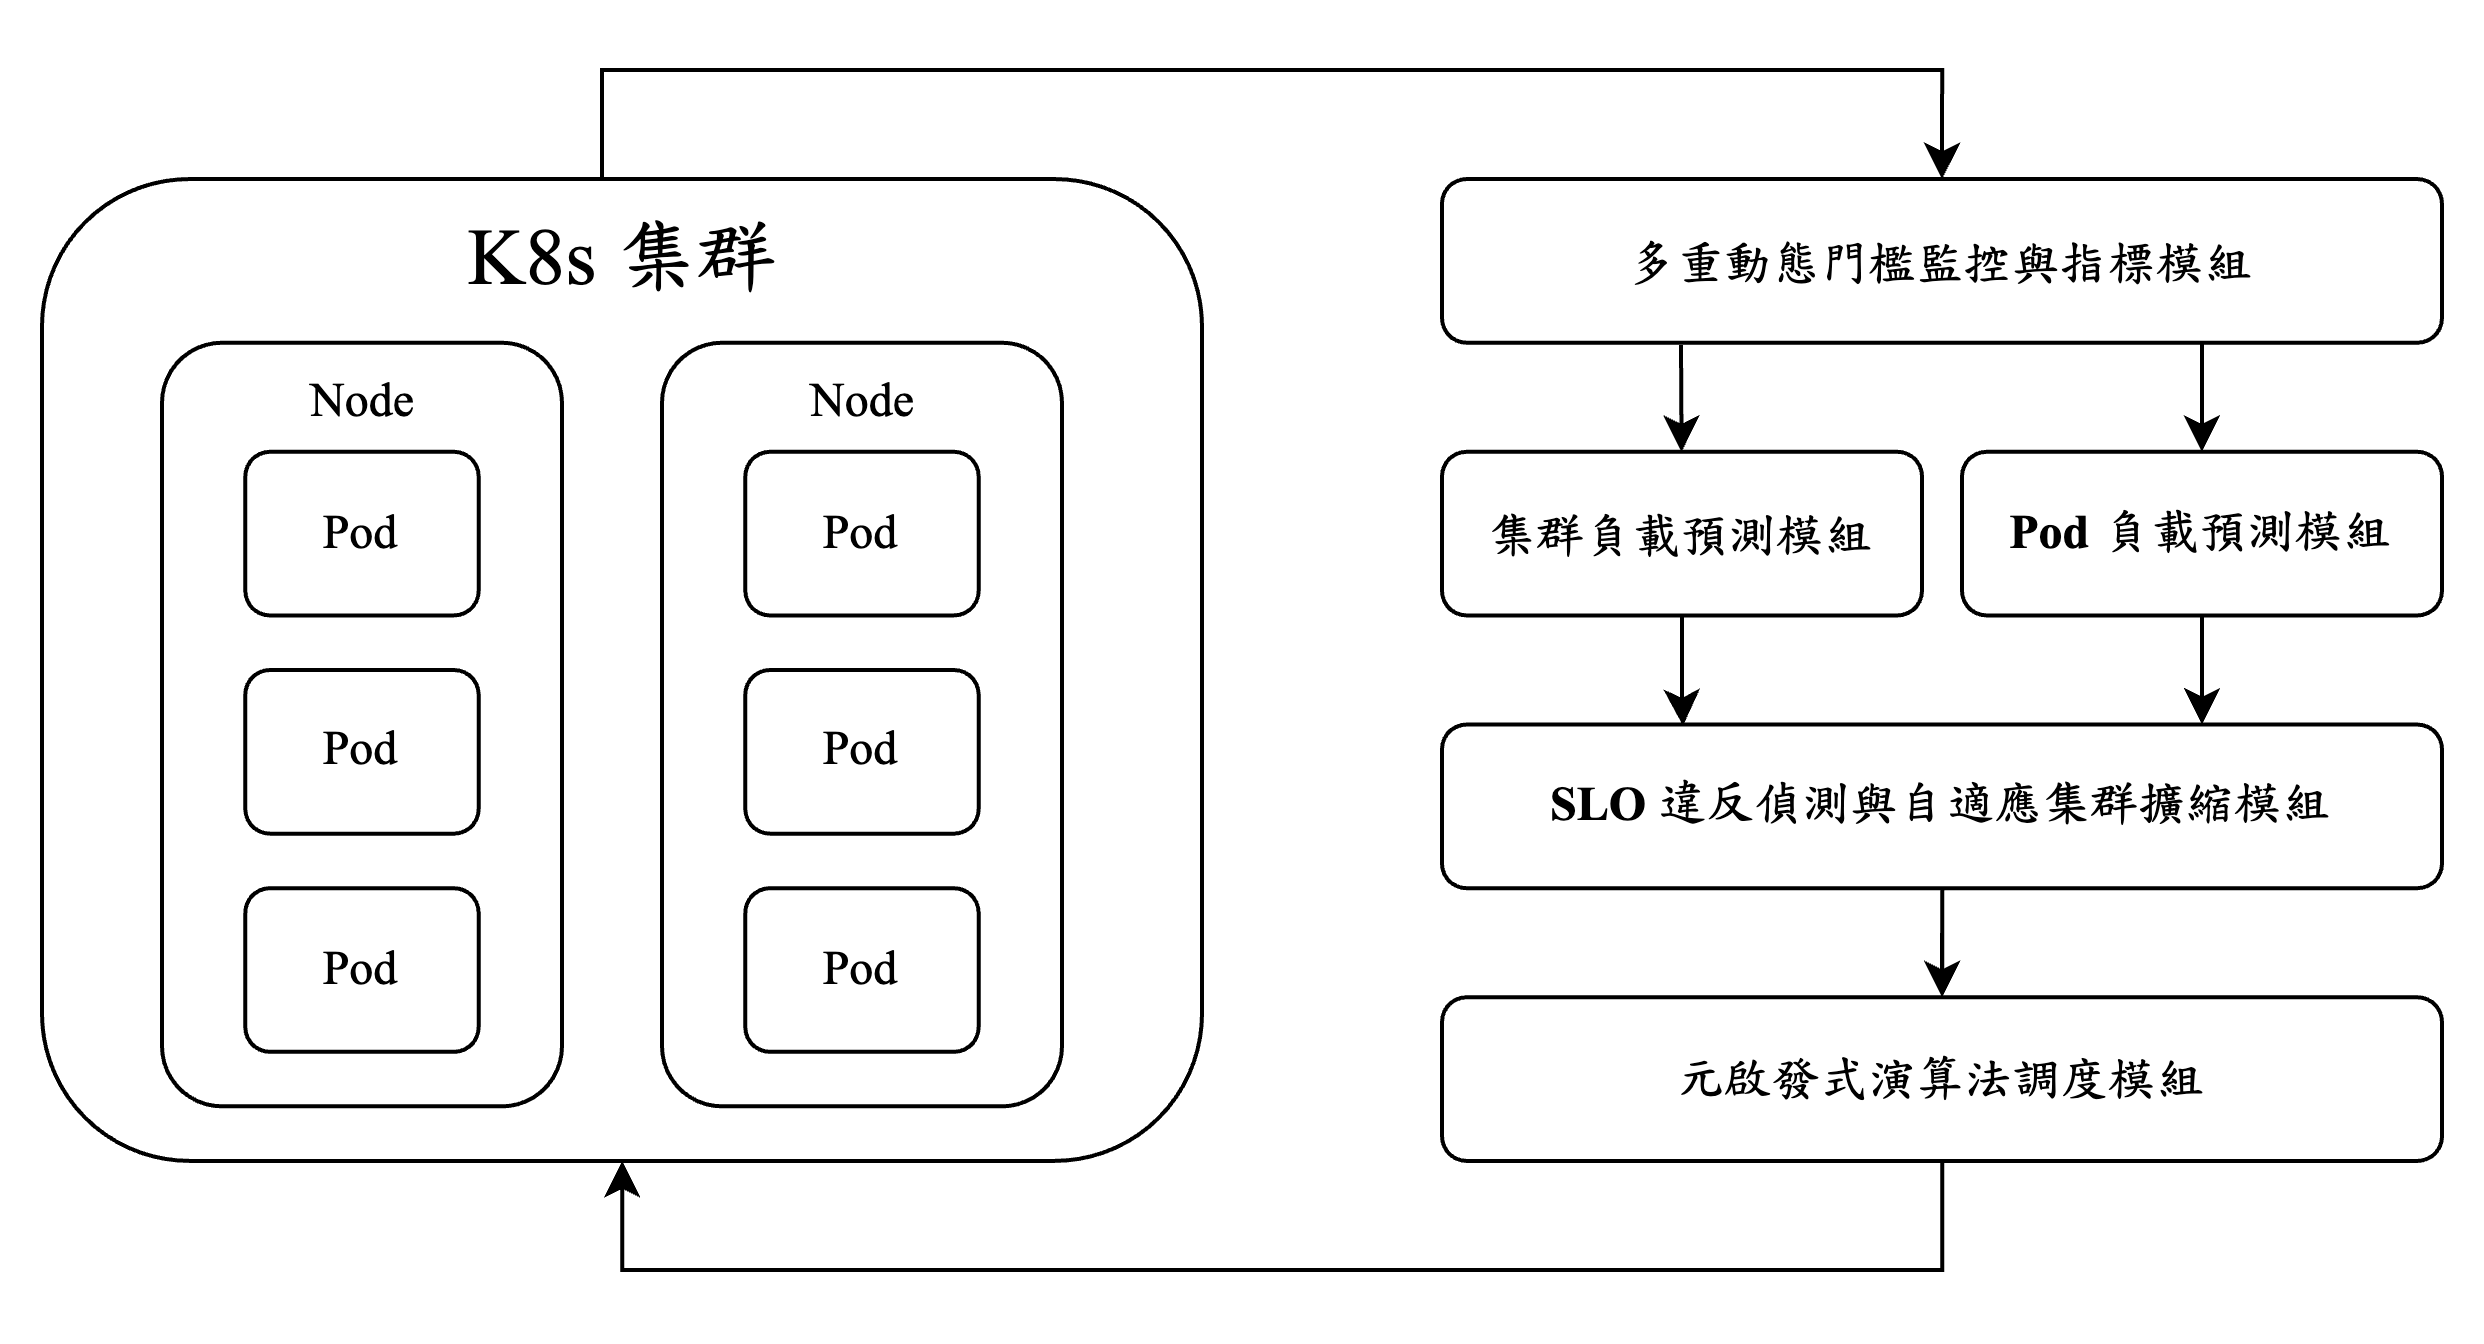
\includegraphics[width=0.9\textwidth]{../figure/model.png}

    \caption{架構示意圖}

\end{figure}\newpage

    \item \textbf{
系統運作流程}

當 API 請求進入 Kubernetes 叢集時,系統將根據 API 負載變化與資源狀況,
進行動態預測、智能調度與自適應擴展,具體流程如下:
\begin{enumerate}[label={(\zhdig*)}, leftmargin=\parindent, listparindent=\parindent]

\item \textbf{外部流量 → API Gateway / Ingress Controller}\textbf{}
    \begin{itemize}[leftmargin=\parindent, listparindent=\parindent]

        \item 使用者或裝置的請求 (API Calls) 進入 \textbf{API Gateway} (或 Ingress),Gateway 會將請求導向對應的 \textbf{Service},再分配至後端多個 \textbf{Pod}。
    \end{itemize}
\item \textbf{Kubernetes Metrics / Logs → 多重動態門檻監控與指標模組}\textbf{}
    \begin{itemize}[leftmargin=\parindent, listparindent=\parindent]

        \item \textbf{Kubernetes API Server} 收集叢集中各 \textbf{Node}、各 \textbf{Pod} 的資源使用狀態 (CPU/記憶體/GPU 使用率、RPS、錯誤率等);同時也可整合 \textbf{Metrics Server}、\textbf{Prometheus} 等第三方監控工具,將資料傳至 \textbf{多重動態門檻監控與指標模組}。

        \item 該模組將這些數據進行整理,並與動態門檻 (SLA 閾值) 比較,判定是否產生 SLO 違反風險。
    \end{itemize}
\item \textbf{歷史負載資料 → CNN/LSTM 預測模型}\textbf{}
    \begin{enumerate}[label={(\arabic*)}, leftmargin=\parindent, listparindent=\parindent]

        \item \textbf{集群負載預測模組 (CNN)}:
        \begin{itemize}[leftmargin=\parindent, listparindent=\parindent]
            \item 從 \textbf{多重動態門檻監控與指標模組} 以及歷史紀錄庫 (Database) 取得「整體叢集級的歷史負載 (e.g. 過去一週的 QPS、CPU 使用率)」,再進行 CNN 預測。

            \item 預測結果 (未來一段時間整體流量或 CPU/記憶體需求) 會回傳給 \textbf{多重動態門檻監控與指標模組},再進一步判斷是否要觸發集群層級擴縮。
        \end{itemize}
        \item \textbf{Pod 負載預測模組 (LSTM)}:
            \begin{itemize}[leftmargin=\parindent, listparindent=\parindent]
                \item 針對單個 Pod / 微服務取得「歷史 RPS、CPU/記憶體使用情況」等資料,進行 LSTM 預測。

                \item 預測結果 (特定服務在未來時段的負載) 也會提供給 \textbf{多重動態門檻監控與指標模組},讓它判定是否需要對該微服務啟動 \textbf{HPA/VPA} 進行水平或垂直擴縮。
            \end{itemize}
    \end{enumerate}
\item \textbf{監控 + 預測 → SLO 違反偵測與自適應集群擴縮模組}\textbf{}
    \begin{itemize}[leftmargin=\parindent, listparindent=\parindent]

        \item 當 \textbf{多重動態門檻監控與指標模組} 發現某些指標逼近閾值,或從 CNN / LSTM 模型得知未來負載將大幅攀升,就會將訊號上報給 \textbf{SLO 違反偵測與自適應集群擴縮模組}。

        \item 該模組會分析「SLO 達成率 (成功率、延遲指標)」與「資源使用現況」之間的落差,若判定「需要擴容」,則呼叫 \textbf{Cluster Autoscaler} 增加 Node;若判定「需要釋放資源」,則啟動縮容程序。但期間可能會搭配「自適應冷卻 (Cooldown)」避免過度頻繁地伸縮。

        \item 同時也可呼叫 \textbf{HPA / VPA},對特定 Pod 增減副本數量或調整單 Pod 資源配額。
    \end{itemize}
\item \textbf{自適應擴縮決策 → 元啟發式演算法調度模組 / 自訂 Kubernetes Scheduler}\textbf{}
    \begin{itemize}[leftmargin=\parindent, listparindent=\parindent]

        \item 當要新建 Pod 或需要重新安排容器時,\textbf{SLO 違反偵測與自適應集群擴縮模組} 會將「建立 Pod」的需求傳給 \textbf{Scheduler}。

        \item 若系統啟用了 \textbf{自訂 Kubernetes Scheduler} (整合基因演算法或其他元啟發式演算法),則會參考目前 Node 資源使用率、網路延遲、預測負載與優先級等資訊,計算哪個 Node 比較適合佈署新的 Pod。

        \item 得到結論後,再由 \textbf{Scheduler} 向 \textbf{API Server} 登記排程決策,最終由 \textbf{Kubelet} 在目標 Node 上啟動容器。
    \end{itemize}
\item \textbf{部署完成 → 持續監控與迴圈}\textbf{}
    \begin{itemize}[leftmargin=\parindent, listparindent=\parindent]

        \item 新增的 Node 或 Pod 就緒 (Ready) 後開始分擔部分流量。

        \item \textbf{多重動態門檻監控與指標模組} 會持續監測系統負載、性能指標,並反饋到預測模型與 \textbf{SLO 違反偵測與自適應集群擴縮模組},形成一個 \textbf{動態自我調整} 的閉環。
\end{itemize}
    \end{enumerate}

\item \textbf{
    系統流程圖}
\begin{figure} [htbp]

    \centering

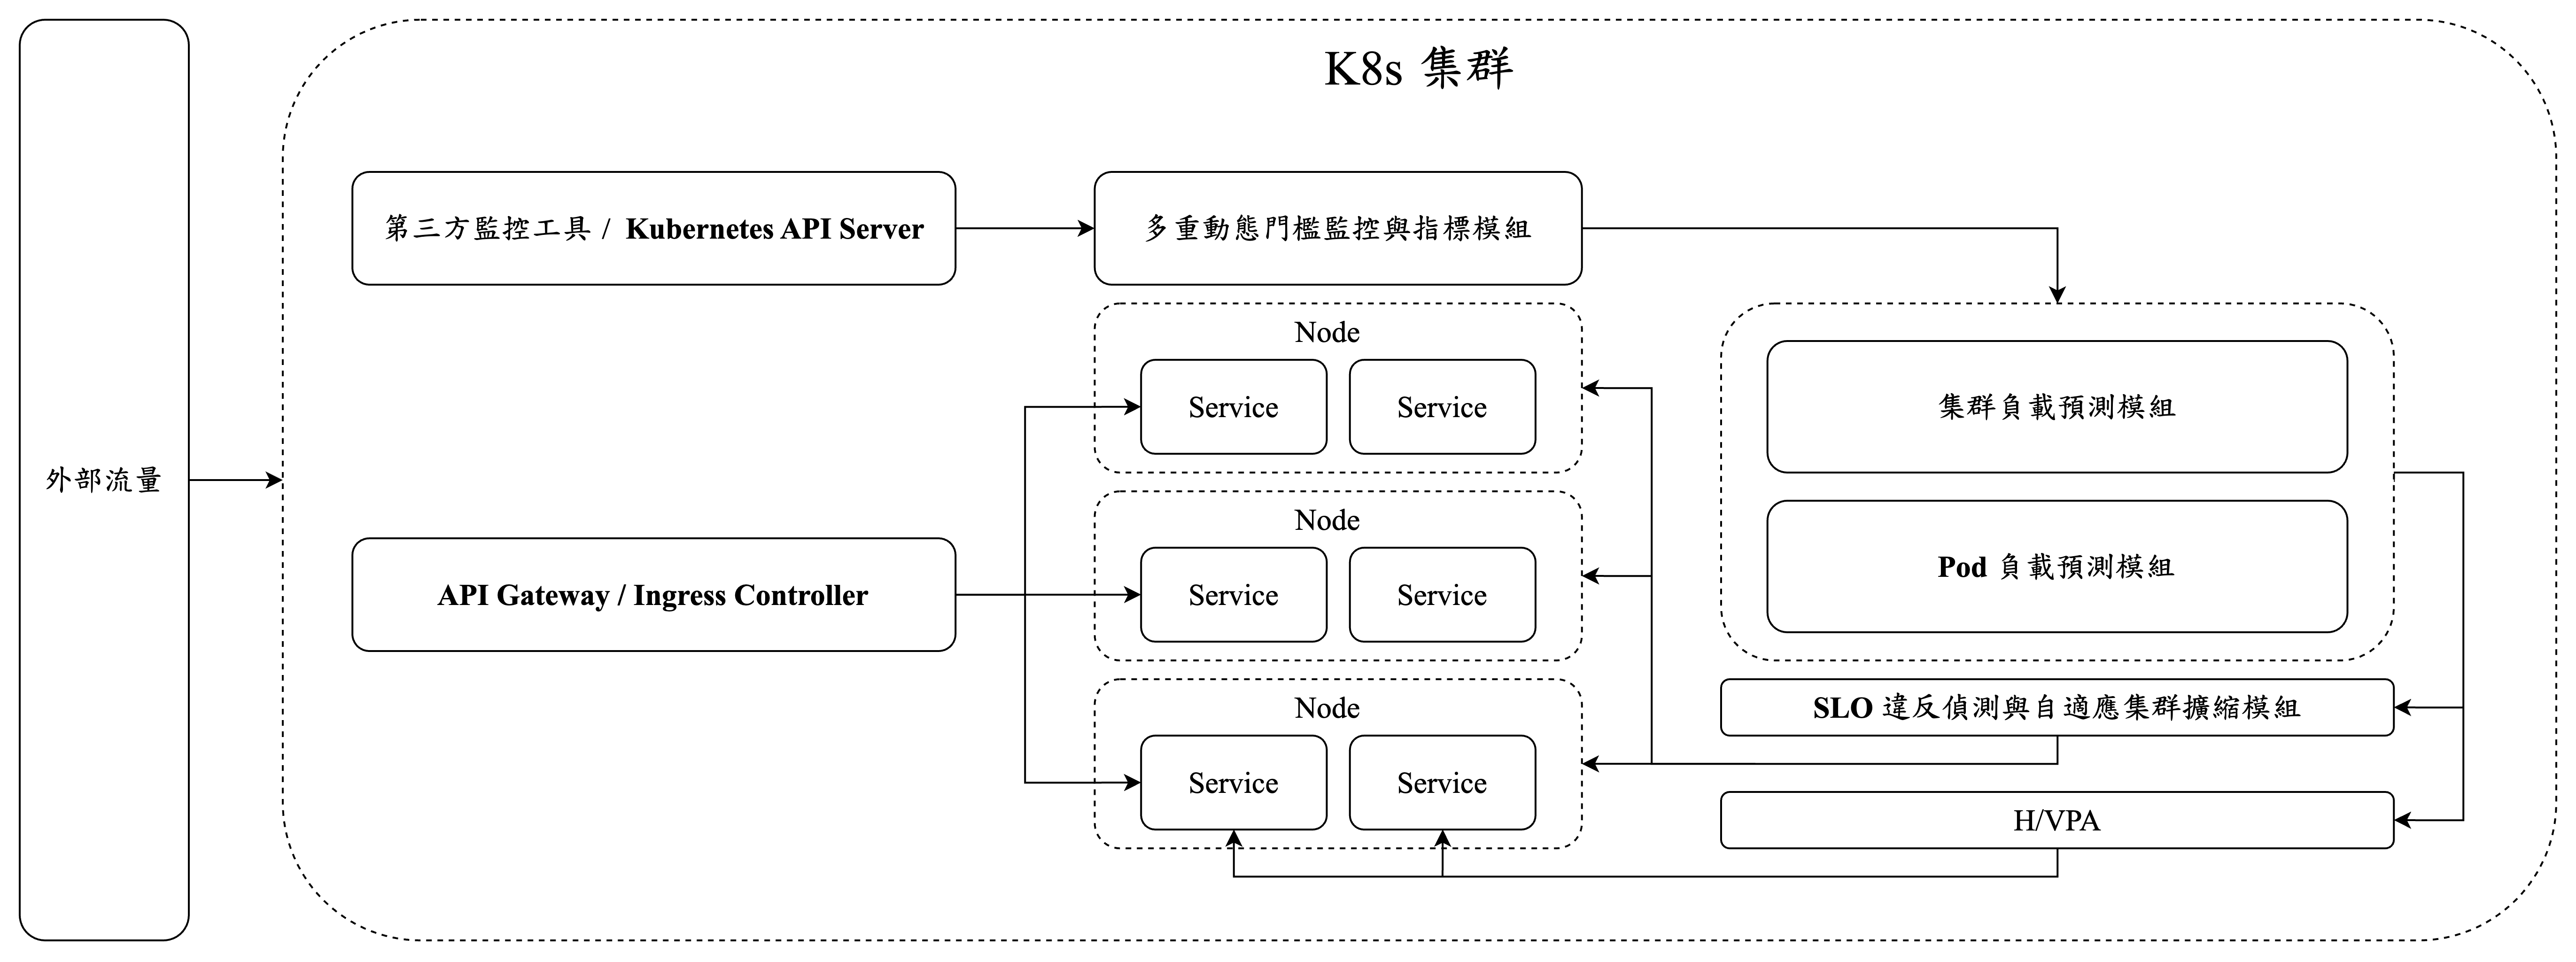
\includegraphics[width=0.9\textwidth]{../figure/flowchart.png}

    \caption{流程示意圖}

\end{figure}

\item \textbf{
    目前研究進度}

    已經架設完畢 Kubernetes 環境並挑選一些微服務來維持集群的負載,並設計完自適應集群擴縮模組與實作進Kubernetes環境中。

\begin{figure} [htbp]

    \centering

    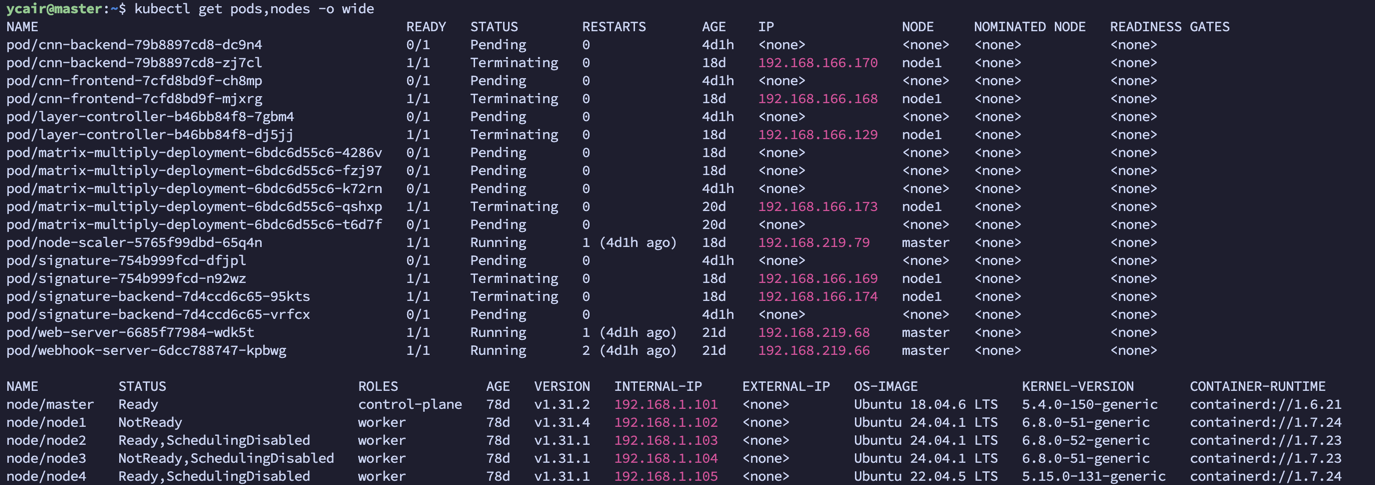
\includegraphics[width=0.9\textwidth]{../figure/k8s.png}

    \caption{Kubernetes 環境示意圖}

\end{figure}

\begin{figure} [htbp]

    \centering

    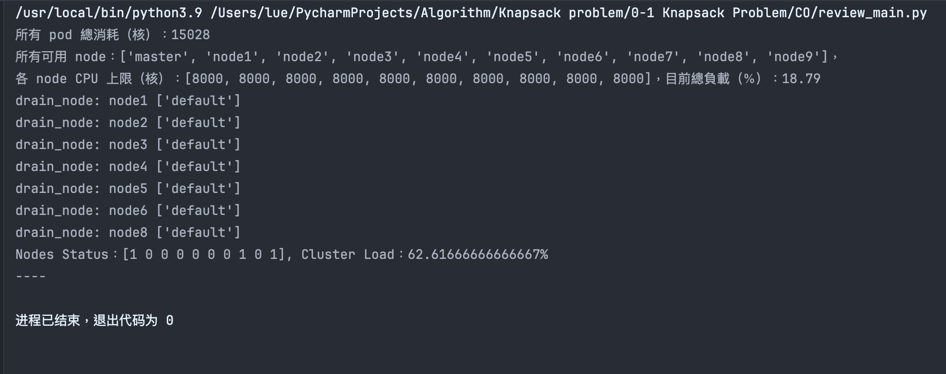
\includegraphics[width=0.9\textwidth]{../figure/CO.png}

    \caption{自適應集群擴縮演算法示意圖}

\end{figure}\newpage

\end{enumerate}
\item 預期結果
\begin{enumerate}[label={(\arabic*)}, leftmargin=\parindent, listparindent=\parindent]
\item \textbf{降低延遲與提升穩定度}\textbf{}

由於系統可在流量飆升前即預測負載並提前擴容,API 請求不易出現塞車情況,使平均響應時間維持在要求的 SLA 閾值之內。

\item \textbf{提高資源利用率並減少成本浪費}\textbf{}

透過 CNN/LSTM 負載預測與自適應擴縮,僅在確有需求時才動態擴增容器或節點,流量回落後則自動縮減,避免長期閒置造成的資源浪費。

\item \textbf{減少 SLO 違反時間}\textbf{}

動態監控機制能即時偵測到服務延遲或成功率下滑的徵兆,並快速啟動相應調度與擴容策略;同時搭配元啟發式演算法優化節點排程,進一步降低違反 SLA 的機率及時間。

\item \textbf{因應高併發場景的彈性擴展}\textbf{}

不論是金融交易、電商促銷或物聯網尖峰時段,本系統都能在秒級到分級內快速分配更多容器、副本或節點,支撐突增的 API 請求量,並在需求趨緩後自動回收,以維持成本效益。

\item \textbf{整體運維效率與可擴充性提升}\textbf{}

結合自動化冷卻機制與 Kubernetes 的自訂排程器,減少了人工調參與嘗試錯誤的過程;同時支援多雲與異構資源環境,利於未來的功能擴充與跨平台部署。
\end{enumerate}

\item 需要指導教授指導內容

\begin{enumerate}[label={(\arabic*)}, leftmargin=\parindent, listparindent=\parindent]

	\item \textbf{實驗環境搭建與平台配置:}\textbf{}
\begin{itemize}[leftmargin=\parindent, listparindent=\parindent]

    \item 指導如何規劃與構建一個能模擬真實高並發情境的實驗環境,包含容器編排平台(例如 Kubernetes)及相關虛擬化資源的配置。


    \item 協助設定網路、存儲與安全機制,確保實驗平台在資源分配與通訊上能夠滿足實驗需求。

\end{itemize}
\item \textbf{高併發流量模擬與負載生成:}\textbf{}

    \begin{itemize}[leftmargin=\parindent, listparindent=\parindent]
        \item 協助設計針對不同流量模式(如突發流量、持續高負載、周期性波動)的模擬方案,並選用合適的壓力測試工具生成大量 API 請求。


        \item 指導如何規劃實驗情境,使測試數據能夠全面反映系統在各種極端負載下的運行情況。

    \end{itemize}
\item \textbf{容器調度算法與自動擴縮策略驗證:}\textbf{}

    \begin{itemize}[leftmargin=\parindent, listparindent=\parindent]
        \item 指導實驗如何針對不同的容器調度演算法進行性能比較,包括調度決策速度、資源利用率以及延遲表現。


        \item 協助設計自動擴縮策略的實驗,驗證在面臨高併發時,系統能否迅速動態調整容器副本數並保持穩定運作。
    \end{itemize}

\item \textbf{負載預測模型與決策機制測試:}\textbf{}

    \begin{itemize}[leftmargin=\parindent, listparindent=\parindent]
        \item 指導如何將深度學習或強化學習模型融入負載預測實驗,並驗證預測結果對調度決策的正向影響。


        \item 協助建立數據收集與分析流程,評估模型在不同負載情境下的預測準確率與實際調度效能的改進幅度。

    \end{itemize}
\item \textbf{系統穩定性與容錯性測試:}\textbf{}

    \begin{itemize}[leftmargin=\parindent, listparindent=\parindent]
        \item 指導設計針對容器故障、網路中斷或資源緊缺等異常情況的測試,驗證系統在面對突發故障時的恢復能力與容錯機制。


        \item 協助規劃測試流程,觀察系統在各類異常狀況下的響應時間、故障切換與自我修復表現。

    \end{itemize}
\item \textbf{實驗數據分析與性能評估:}\textbf{}

    \begin{itemize}[leftmargin=\parindent, listparindent=\parindent]
        \item 指導如何統整並分析各項測試數據,從中評估系統在高併發環境下的整體調度效能、響應延遲與資源分配效率。


        \item 協助制定具體的評估指標,並針對實驗結果撰寫數據分析報告,找出系統瓶頸與優化方向。

    \end{itemize}
\item \textbf{實驗結果展示與驗證論證:}\textbf{}

    \begin{itemize}[leftmargin=\parindent, listparindent=\parindent]
        \item 指導如何使用圖表、統計分析等方法清晰呈現實驗結果,驗證系統架構在高並發情境下的優勢。


        \item 協助論證實驗數據與預期目標的吻合程度,並提出後續改進與優化策略的建議。
    \end{itemize}
\end{enumerate}
\item 參考文獻

\printbibliography[heading=none]

\end{enumerate}


\label{LastPage}


\end{document}

